%appendix B
%p_storage

\section{Overview}
\begin{figure}[ht]
    \centering
    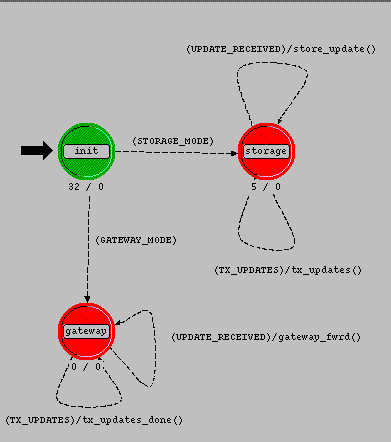
\includegraphics[scale=0.5]{images/p_storage}
    \caption{Storage process model}
    \label{fig:appendix-b}
\end{figure}

\newpage

\section{Local variables}
\begin{figure}[h]
    \centering
    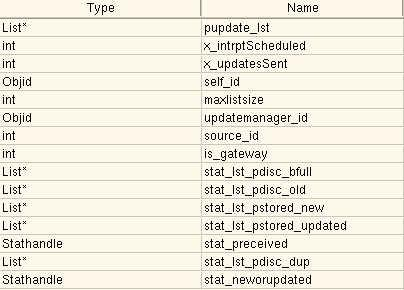
\includegraphics[width=.7\textwidth]{images/state_variable_storage}
    \caption{State variables of storage process}
    \label{fig:appendix-b_sv}
\end{figure}

\section{Header Block}
%_____________________________________HEADER______________________________________
{\tiny
\begin{verbatim}
#define MAX_SRC_IDS		10
#define GATEWAY_MODE	(is_gateway)
#define STORAGE_MODE	(!GATEWAY_MODE)
#define STRM_UM_IN		0
#define STRM_UM_OUT		0
#define STRM_GW_OUT		1
//Interrupt Codes (random numbers)
#define IC_DUMP_UPDATES 		73
#define IC_DUMP_UPDATES_DONE 	74
#define IC_SOURCPROP_ACTION 99
#define TX_UPDATES 		(op_intrpt_type() == OPC_INTRPT_REMOTE && op_intrpt_code() == IC_DUMP_UPDATES)
#define UPDATE_RECEIVED	(op_intrpt_type() == OPC_INTRPT_STRM)

int written_global_storage_stat = 0;
List *create_stat_lst_loc(const char *);
void store_update(void);
void tx_updates(void);
void gateway_fwrd(void);
\end{verbatim}
}

\section{Function Block}
%______________________________FUNCTION__________________________________
{\tiny
\begin{verbatim}
void store_update(void)
{
	Packet *pkt;
	Packet *lstPkt;
	char message_str [255];
	Objid prop1_id;
	int key;
	int sourceid;
	int key_updnm;
	int pos_index;
	double gen_ts;
	int newkey;
	int newsourceid;
	int newkey_updnm;
	double newgen_ts;
	int listsize;
	int i, j, k;
	double temp;
	Ici *iciptr;
	Objid source_prop_id;	
	FIN (store_update ());
	pkt = op_pk_get (op_intrpt_strm ());
	
	//get info
	op_pk_nfd_get(pkt, "key", &newkey);
	op_pk_nfd_get(pkt, "source_id", &newsourceid);
	op_pk_nfd_get(pkt, "key_update_number", &newkey_updnm);
	op_pk_nfd_get(pkt, "generated_timestamp", &newgen_ts);
	listsize = op_prg_list_size(pupdate_lst);
	
	if(newsourceid < 0 || newsourceid >= MAX_SRC_IDS)
	{
		op_sim_end("Bad sourceid", "", "", "");
	}
	op_stat_write(stat_preceived, 1.0);
	
	//Search & Compare 'key_update_number'; replace if newer
	for(i = 0; i < listsize; i++)
	{
		lstPkt = (Packet *)op_prg_list_access (pupdate_lst, i);
		op_pk_nfd_get(lstPkt, "key", &key);
		op_pk_nfd_get(lstPkt, "source_id", &sourceid);
		op_pk_nfd_get(lstPkt, "key_update_number", &key_updnm);
		op_pk_nfd_get(lstPkt, "generated_timestamp", &gen_ts);
	
		//COMPARE for matching source/key
		if(newsourceid == sourceid)
		{
			if(newkey == key)
			{
				if(newkey_updnm > key_updnm)	//if key is newer we update
				{
					if(newsourceid != source_id)
					{
						op_stat_write(*((Stathandle *)op_prg_list_access (stat_lst_pstored_updated, sourceid)), 1.0);
						op_stat_write(stat_neworupdated, 1.0);
					}
					op_pk_nfd_get(lstPkt, "source_prop_objid", &source_prop_id);
					iciptr = op_ici_create ("prop_action");
					op_ici_attr_set (iciptr, "source_id", sourceid);
					op_ici_attr_set (iciptr, "key_update_number", newkey_updnm);
					op_ici_attr_set (iciptr, "action", 2);
					op_ici_install(iciptr);
					op_intrpt_schedule_remote (op_sim_time (), IC_SOURCPROP_ACTION, source_prop_id);

					iciptr = op_ici_create ("prop_action");
					op_ici_attr_set (iciptr, "source_id", sourceid);
					op_ici_attr_set (iciptr, "key_update_number", key_updnm);
					op_ici_attr_set (iciptr, "action", 3); //3 = discard
					op_ici_attr_set (iciptr, "discard_reason", 1); //1 = update
					op_ici_install(iciptr);
					op_intrpt_schedule_remote (op_sim_time (), IC_SOURCPROP_ACTION, source_prop_id);
										
					op_prg_list_remove (pupdate_lst, i);
					op_prg_list_insert(pupdate_lst, pkt, OPC_LISTPOS_TAIL);
					op_pk_destroy(lstPkt);
					FOUT;
				}
				else
				{
					if(newkey_updnm == key_updnm)
					{
						op_stat_write(*((Stathandle *)op_prg_list_access (stat_lst_pdisc_dup, sourceid)), 1.0);
					}
					else
					{
						op_stat_write(*((Stathandle *)op_prg_list_access (stat_lst_pdisc_old, sourceid)), 1.0);
					}
					//Dont need to trigger the source prop intrupt because this pkt was never stored
					op_pk_destroy(pkt);
					FOUT;
				}
			}
		}
	} //forloop

	op_pk_nfd_get(pkt, "source_prop_objid", &source_prop_id);				
	iciptr = op_ici_create ("prop_action");
	op_ici_attr_set (iciptr, "source_id", newsourceid);
	op_ici_attr_set (iciptr, "key_update_number", newkey_updnm);
	op_ici_attr_set (iciptr, "action", 2); //2 = store
	op_ici_install(iciptr);
	op_intrpt_schedule_remote (op_sim_time (), IC_SOURCPROP_ACTION, source_prop_id);
	op_prg_list_insert(pupdate_lst, pkt, OPC_LISTPOS_TAIL);
	listsize = op_prg_list_size(pupdate_lst);

	if(newsourceid != source_id)
	{
		op_stat_write(*((Stathandle *)op_prg_list_access (stat_lst_pstored_new, newsourceid)), 1.0);
		op_stat_write(stat_neworupdated, 1.0);
	}
	//See if we need to get rid of something
	if(listsize > maxlistsize)
	{	
		//set first packet for temp
		lstPkt = (Packet *)op_prg_list_access (pupdate_lst, 0);
		op_pk_nfd_get(lstPkt, "generated_timestamp", &gen_ts);
		temp = gen_ts;
		
		//find oldest timestamp
		for(j = 0; j < listsize; j++)
		{
			lstPkt = (Packet *)op_prg_list_access (pupdate_lst, j);
			op_pk_nfd_get(lstPkt, "generated_timestamp", &gen_ts);		
			if(gen_ts < temp)
			{
				temp = gen_ts;	//replace if older
			}
		}
	
		//delete packet with oldest timestamp, temp, 
		for(k = 0; k < listsize; k++)
		{
			lstPkt = (Packet *)op_prg_list_access (pupdate_lst, k);
			op_pk_nfd_get(lstPkt, "generated_timestamp", &gen_ts);
			op_pk_nfd_get(lstPkt, "source_id", &sourceid);
			op_pk_nfd_get(lstPkt, "key_update_number", &key_updnm);
			
			if(temp == gen_ts)
			{
				op_stat_write(*((Stathandle *)op_prg_list_access (stat_lst_pdisc_bfull, sourceid)), 1.0);
				op_pk_nfd_get(lstPkt, "source_prop_objid", &source_prop_id);				
				iciptr = op_ici_create ("prop_action");
				op_ici_attr_set (iciptr, "source_id", sourceid);
				op_ici_attr_set (iciptr, "key_update_number", key_updnm);
				op_ici_attr_set (iciptr, "action", 3); //3 = discard
				op_ici_attr_set (iciptr, "discard_reason", 2); //2 = Memory Full
				op_ici_install(iciptr);
				op_intrpt_schedule_remote (op_sim_time (), IC_SOURCPROP_ACTION, source_prop_id);				
				op_prg_list_remove (pupdate_lst, k);
				op_pk_destroy(lstPkt);

				break;
			}
		}
	}
	FOUT;
}
void tx_updates(void)
{
	int i;
	int lstSize;
	Packet *pkt;
	Packet *pPktCopy;
	char message_str [255];	
	FIN (tx_updates ());
	
	lstSize = op_prg_list_size (pupdate_lst);
	for (i = 0; i < lstSize; i++)
	{
		pkt = (Packet *) op_prg_list_access (pupdate_lst, i);		
		pPktCopy = op_pk_copy(pkt);
		op_pk_send(pPktCopy, STRM_UM_OUT);
	}
	op_intrpt_schedule_remote(op_sim_time(), IC_DUMP_UPDATES_DONE, updatemanager_id);
	FOUT;
}
void tx_updates_done(void)
{
	FIN (tx_updates_done ());	
	op_intrpt_schedule_remote(op_sim_time(), IC_DUMP_UPDATES_DONE, updatemanager_id);
	FOUT;
}
void gateway_fwrd()
{
	FIN (update_gateway ());
	op_stat_write(stat_preceived, 1.0);
	op_pk_send(op_pk_get(STRM_UM_IN), STRM_GW_OUT);
	FOUT;
}
List *create_stat_lst_loc(const char *statName)
{
	List *lst;
	int stat_size_asdf;
	int i;
	char msg1[255];
	char msg2[255];
	
	FIN(create_stat_lst_loc());	
	op_stat_dim_size_get(statName, OPC_STAT_LOCAL, &stat_size_asdf);
	if(stat_size_asdf != MAX_SRC_IDS)
	{
		sprintf(msg1, "stat_size_asdf: %d", stat_size_asdf);
		sprintf(msg2, "MAX_SRC_IDS: %d", MAX_SRC_IDS);
		op_sim_end("Bad stat dimension", statName, msg1, msg2);
	}
	lst = op_prg_list_create();
	for(i = 0; i < MAX_SRC_IDS; i++)
	{
		Stathandle *sth_temp;
		sth_temp = (Stathandle *) op_prg_mem_alloc (sizeof (Stathandle));
		*sth_temp = op_stat_reg (statName, i, OPC_STAT_LOCAL);
		
		op_prg_list_insert(lst, sth_temp, OPC_LISTPOS_TAIL);
	}
	FRET(lst);
}
\end{verbatim}
}

\section{init State: Enter Executives}
%______________________________________Init_____________________________________________________________
{\tiny
\begin{verbatim}
int i;
self_id = op_id_self();
printf("REGISTERING STATS\n");
stat_lst_pstored_new = create_stat_lst_loc("Pkts Stored - New");
stat_lst_pstored_updated = create_stat_lst_loc("Pkts Stored - Updated");
stat_lst_pdisc_old = create_stat_lst_loc("Pkts Discarded - Old");
stat_lst_pdisc_bfull = create_stat_lst_loc("Pkts Discarded - Buffer Full");
stat_lst_pdisc_dup = create_stat_lst_loc("Pkts Discarded - Duplicate");
stat_preceived = op_stat_reg("Pkts Received",OPC_STAT_INDEX_NONE, OPC_STAT_LOCAL);
stat_neworupdated = op_stat_reg("Pkts Stored - New or Updated",OPC_STAT_INDEX_NONE, OPC_STAT_LOCAL);

pupdate_lst = op_prg_list_create (); 		//allocate an empty list
op_ima_sim_attr_get (OPC_IMA_INTEGER, "Capacity", &maxlistsize);
if(written_global_storage_stat == 0)
{
	written_global_storage_stat = 1;
	op_stat_write_scalar("Storage Capacity", maxlistsize);
}
op_ima_obj_attr_get (self_id, "Source ID", &source_id);
op_ima_obj_attr_get (self_id, "Is Gateway", &is_gateway);
updatemanager_id = op_id_from_name (op_topo_parent(self_id), OPC_OBJTYPE_PROC, "update_manager");
\end{verbatim}
}

\section{storage State: Enter Executives}
%______________________________________Storage_____________________________________________________________
{\tiny
\begin{verbatim}
if(maxlistsize <= 0)
{
	//Typically when this node is a gateway
	op_sim_end("Invalid max list size", "", "", "");
}
\end{verbatim}
}
